\documentclass[a4paper,11pt]{article}
\usepackage{graphicx}
\usepackage{enumerate}
\usepackage[usenames, dvipsnames]{color}

\begin{document}

\begin{flushright}

\vspace{1.1cm}

{\bf\Huge Problem Set 6}

\rule{0.25\linewidth}{0.5pt}

\vspace{0.5cm}
%Put Authors
Justin Ely
\linebreak
\newline
%Put Author's affiliations
\footnotesize{605.411 Foundations of Computer Architecture \\}
\vspace{0.5cm}
% Date here below
11 October, 2016
\end{flushright}

\noindent\rule{\linewidth}{1.0pt}

%%%%%%%%%%%%%%%%%%%%%%%%%%%%%%%%%%%%%%%%%%%%%%%%%%%%%%%%%%

\section*{1a)}
\begin{tabular}{| c | c |}
  \hline	
  	Op & Cycles \\ \hline \hline
	or & 4 \\ \hline
	and & 4 \\ \hline
	sub & 4 \\ \hline
	sw & 4 \\ \hline
	lw & 5 \\ \hline
	add & 4 \\ \hline
	bne & 3 \\ \hline \hline
	Total & 28 \\ \hline
\end{tabular} \\

\section*{1b)}
For a single-cycle datapath, each instruction must use all 5 stages.  This makes the total time 11ns.  The clock rate is then
$\frac{1}{11e-9} = 90.0MHz$.

\section*{1c)}
In a 5-stage pipeline, each instruction will use all 5 stages and each stage will be the length of the longest stage.  This means the clock cycle is $5ns = 200Mhz$.

\section*{1d)}
Assuming full forwarding, the only command to cause a delay will be the LW, which will cause a delay of 2 cycles.  Thus, the total number of cycles will be 13. 

%%%%%%%%%%%%%%%%%%%%%%%%%%%%%%%%%%%%%%%%%%%%%%%%%%%%%%%%%%

\section*{2a)} 
In a pipelined architecture, the clock cycle time is the same as the longest stage.  For this example, this would be the MEM stage, which is
600ps.

\section*{2b)}
In a single-cycle datapath, the clock cycle time is the sum of all 5 stages = 1500ps.

\section*{2c)}
In a pipelined processor, the latency of an r-type instruction is $600 \times 5 = 3000 ps$ since even an r-type needs to go through all 5 stages.
In a single-cycle processor, the latency of an r-type instruction is the same as the clock cycle time, 1500ps, since each instruction executes in 1 cycle.

%%%%%%%%%%%%%%%%%%%%%%%%%%%%%%%%%%%%%%%%%%%%%%%%%%%%%%%%%%

\section*{3)}
$\frac{\frac{1}{70 \times 1e6}}{n_{stages}} = 4e-9$  thus $n_{stages} = 3.57$.  This means 4 stages will be needed, as fractional stages
are impossible.  

%%%%%%%%%%%%%%%%%%%%%%%%%%%%%%%%%%%%%%%%%%%%%%%%%%%%%%%%%%

\section*{4a)}
With no forwarding, and each instruction being dependent on the previous, two bubbles will need to be inserted after each instruction to 
ensure correct operations.  This is because each instruction cannot execute until the previous has finished the WB stage.

\begin{figure}[h!]
\caption{Cycle table for problem 4a.} 
\centering
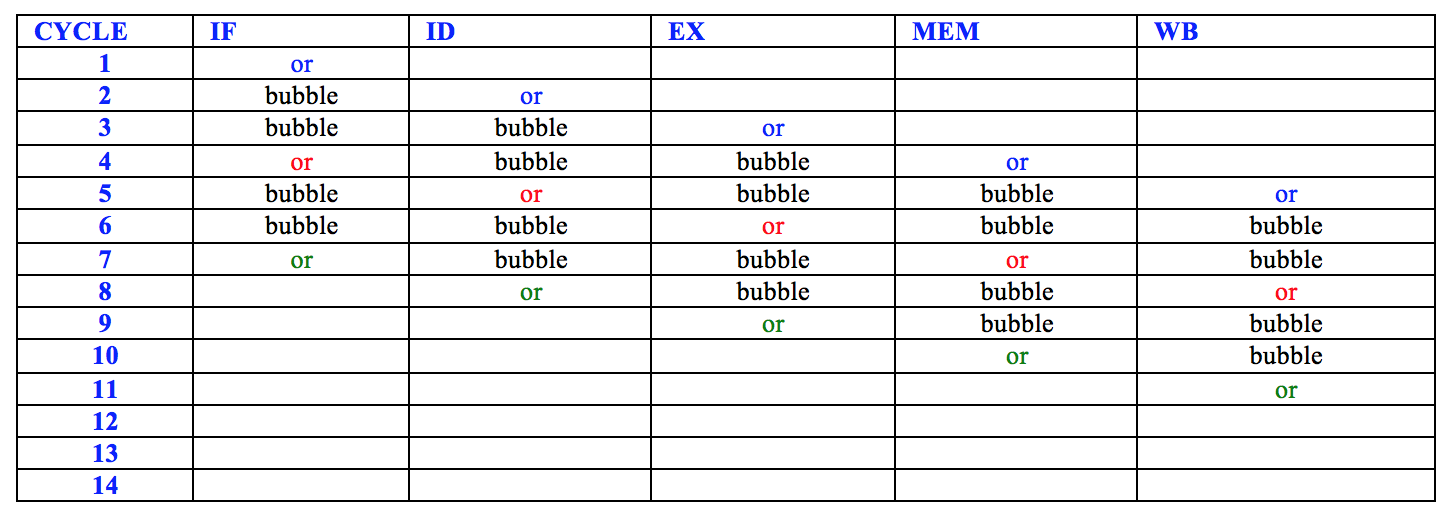
\includegraphics[width=1.1\textwidth]{hw6_p4a.png}
\end{figure}

\section*{4b)}
With full forwarding, all data hazards for sequential r-type instructions are alleviated.

\begin{figure}[h!]
\caption{Cycle table for problem 4b.} 
\centering
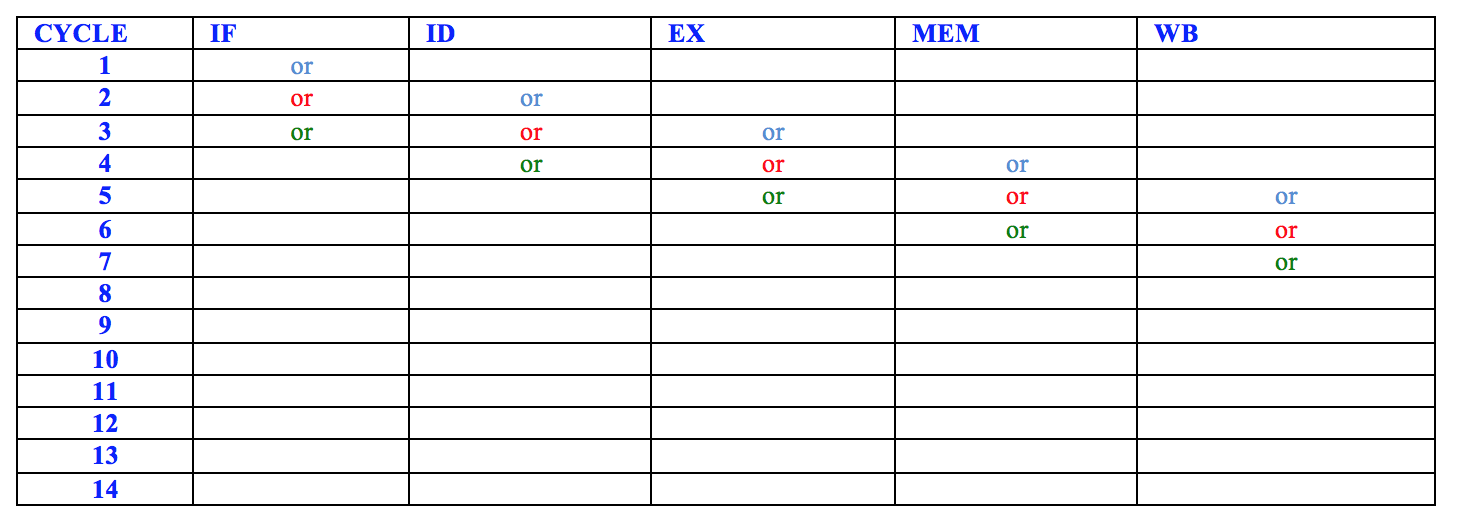
\includegraphics[width=1.1\textwidth]{hw6_p4b.png}
\end{figure}

\section*{4c)}
$\frac{11}{7} = 1.57 $

%%%%%%%%%%%%%%%%%%%%%%%%%%%%%%%%%%%%%%%%%%%%%%%%%%%%%%%%%%

\section*{5)}
With full forwarding, LW and the branch assumption can cause bubbles.  In this example, the branch will be assumed not taken.  
However, upon execution the comparison will be found to be equal and the branch will need to be taken.  

\begin{figure}[h!]
\caption{Cycle table for problem 5.} 
\centering
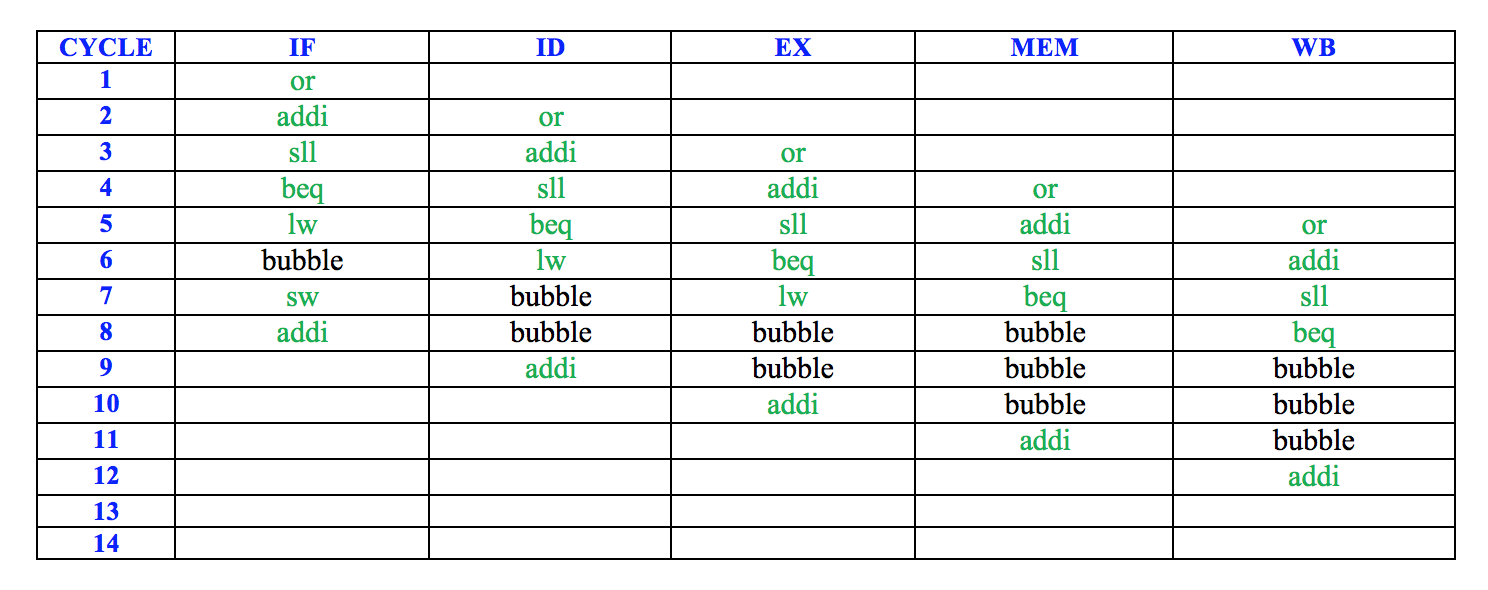
\includegraphics[width=1.1\textwidth]{hw6_p5.png}
\end{figure}

%%%%%%%%%%%%%%%%%%%%%%%%%%%%%%%%%%%%%%%%%%%%%%%%%%%%%%%%%%

\section*{6)}
With full forwarding, the only instruction that will result in a delay is the LW instruction.  A LW followed by an instruction that
requires the loaded word will need to be delayed by one cycle. 

\begin{figure}[h!]
\caption{Cycle table for problem 6.} 
\centering
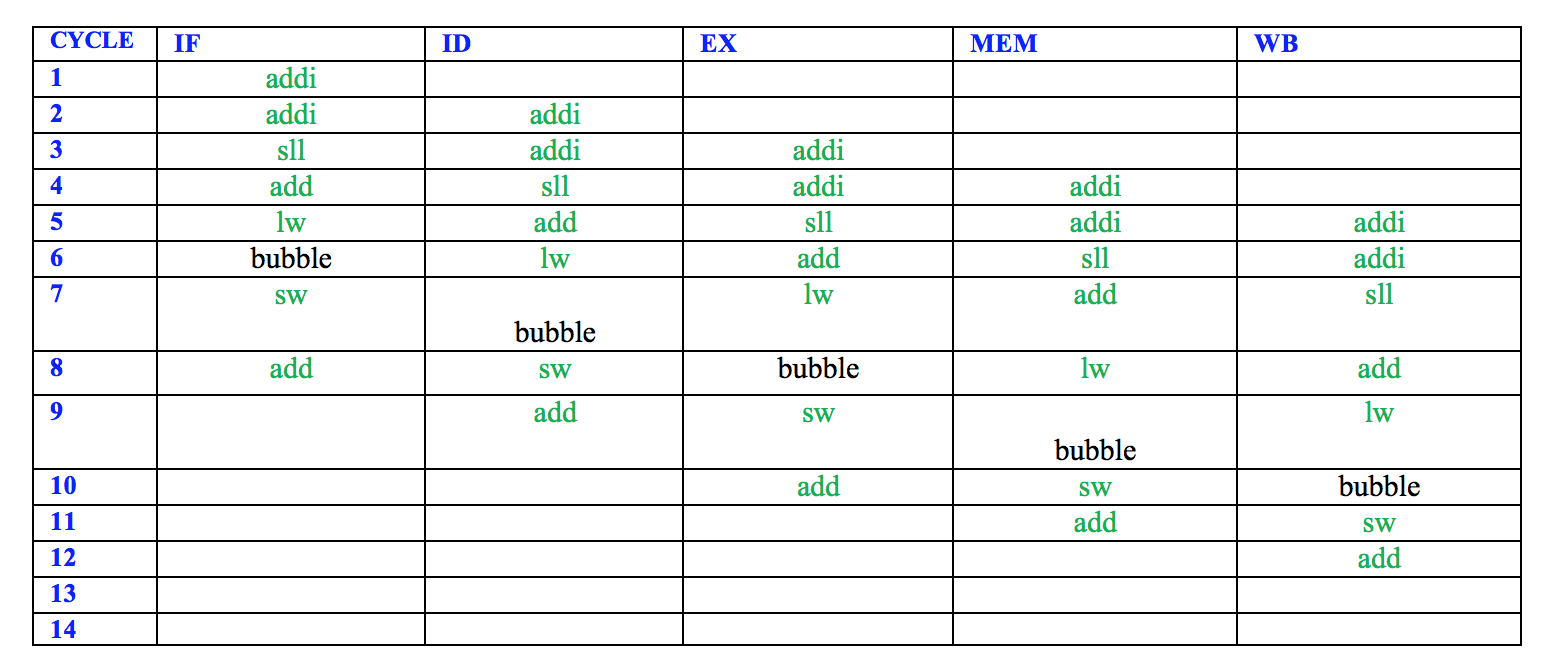
\includegraphics[width=1.1\textwidth]{hw6_p6.png}
\end{figure}

%%%%%%%%%%%%%%%%%%%%%%%%%%%%%%%%%%%%%%%%%%%%%%%%%%%%%%%%%%

\end{document}
